%% uctest.tex 11/3/94
%% Copyright (C) 1988-2004 Daniel Gildea, BBF, Ethan Munson.
%
% This work may be distributed and/or modified under the
% conditions of the LaTeX Project Public License, either version 1.3
% of this license or (at your option) any later version.
% The latest version of this license is in
%   http://www.latex-project.org/lppl.txt
% and version 1.3 or later is part of all distributions of LaTeX
% version 2003/12/01 or later.
%
% This work has the LPPL maintenance status "maintained".
% 
% The Current Maintainer of this work is Daniel Gildea.

\documentclass[11pt,proposal]{ucthesis}
\def\dsp{\def\baselinestretch{2.0}\large\normalsize}
\dsp

% 2010june01 sol katzman:
% package geometry should override the various margin settings from .clo and .cls
% and also eliminates issues where the default papersize is A4
\usepackage[letterpaper, left=1.5in, right=1.25in, top=1.25in, bottom=1.25in, includefoot]{geometry}

\usepackage{url}
\usepackage{listings}
\usepackage{graphicx}

\begin{document}

% Have a command for vocab words
\newcommand{\vocab}[1]{\textbf{#1}}

% Declarations for Front Matter

\title{Infrastructure for Scalable Analysis of Genomic Variation}
\author{Adam M. Novak}
\degreeyear{2014}
\degreemonth{June}
\degree{DOCTOR OF PHILOSOPHY}
\chair{Professor Josh Stuart}
\committeememberone{Professor David Haussler}
\committeemembertwo{Professor Ed Green}
\committeememberthree{Professor Lise Getoor}
\numberofmembers{4} %% (including chair) possible: 3, 4, 5, 6
\deanlineone{Dean \textbf{TODO FIXME}}
\deanlinetwo{Vice Provost and Dean of Graduate Studies}
\deanlinethree{}
\field{Bioinformatics}
\campus{Santa Cruz}

\begin{frontmatter}

\maketitle
\copyrightpage

\tableofcontents
\listoffigures
\listoftables

\begin{abstract}

\end{abstract}

\begin{acknowledgements}

\end{acknowledgements}

\end{frontmatter}

\chapter{Introduction}

Biology happens at scale. Scale in population and in time give evolution the raw materials it needs to shape biological systems worth studying. Scale enables bacteria to become resistant to antibiotics. Scale allows cancer to arise with alarming regularity in healthy people. Scale powers the adaptive immune system, and simultaneously enables pathogens to evade it. To really understand biological systems, we need to be able to match their scale.

In recent years, in part due to a precipitous drop in the cost of DNA sequencing, the scale of biological data collection has dramatically increased \cite{wetterstrand2014dna}. Unfortunately, it has increased disproportionately along the ``number of features'' axis, as opposed to the ``number of samples'' axis. The Cancer Genome Atlas, for example, has collected many types of data, including genomic DNA sequences, DNA methylation data, and mRNA expression levels, amounting to millions of features per sample \cite{tcga2014sample}. However, it has looked at a number of individual people and cancers only on the order of thousands \cite{tcga2014sample}. Similarly, while the 1000 Genomes Project found millions of unique genomic variants, it examined only on the order of a thousand individuals \cite{10002010map}. While such sample sizes may sound large to those who remember the years of effort and multi-billion-dollar expenditure required by the original Human Genome Project, they are woefully small compared to the numbers of features per sample. From a machine learning perspective, this limits the amount of useful knowledge that can be extracted from all of that data. If a theory is to be expected to generalize to new data (that is, if it is to actually reflect the biological processes at work), it generally ought to be based on more data points than features \cite{hua2005optimal}.

For now, it is still possible to use such small sample sizes to do meaningful biology \cite{weinstein2013cancer}. However, at some point in the future, we will exhaust what we can learn by combining our prior knowledge of genetics and biochemistry with a few thousand high-throughput sequencing samples, and we will need to scale up data collection and data analysis in terms of number of samples.

Unfortunately, to scale by even a few orders of magnitude in sample sizes, the way bioinformatics is done will need to change. As it is, working on huge datasets like the sequencing reads from TCGA can be an enormous challenge at the merely technical level, with thousands of gigabytes of data to transfer, store, and protect from unauthorized access. Even lifting over such a huge data set to the new build of the reference genome is going to be a formidable task.

At some point, as we increase the number of samples, we will have to abandon the idea that every lab that wants to analyze these enormous community data sets ought to have its own local copy.

Moreover, when we start to scale up to large numbers of samples, our data sets are more likely to contain individuals who are in some way out of the ordinary, and consequently our engineering standards need to be tightened. For example, if a bioinformatics analysis pipeline assumes that a certain run of genes occur in a certain order and orientation, an increased number of samples pushed through this pipeline translates into an increased chance of encountering an individual who contradicts that assumption, resulting in at best a run-time error and an unhappy bioinformaticist, and at worst a subtly incorrect result in a published paper. All the corner cases---the pathological combinations of variants that we just assume won't occur, or the genomic regions that we would rather not talk about---need to be found and addressed if bioinformatic analyses are going to be made to scale to the sizes they need to scale to.

This means that in order to scale up bioinformatics, we will need to solve a software quality problem. It takes more robust software to handle a million samples than to handle a thousand samples. One way to try to solve this problem might be to make bioinformaticists into better software engineers. A better approach might be to provide them with more robust and more complete software libraries, which provide abstractions that can safely be applied to large numbers of samples, and which consistently expose the now-relatively-frequent edge cases which bioinformaticists will need to deal with at these scales. This latter approach is the one that I intend to take.

One of the abstractions which unfortunately cannot be safely applied at these scales is the idea, central to current bioinformatics practice, of a universal human reference genome and its associated linear coordinate space. When you have only one sequenced genome, it's perfectly reasonable to do things like extract a 2 kilobase window of sequence centered on an arbitrary position. However, we now have a reasonable number of sequenced genomes---enough to get a sense of what common variation exists in the human population, although not enough to understand the significance of many of these \cite{10002010map}---and it is growing increasingly clear that that sort of operation only makes sense in certain cases. In the latest release of the human reference genome, hg38, there are 261 ``alt loci'', or pieces of sequence which are not on the main reference chromosomes, but which model arrangements of genes and other genomic elements which are present in a non-negligible fraction of people \cite{karolchik2014new}. In genomic regions where these alternate haplotypes apply, the traditional linear coordinate system, which refers to locations in peoples' genomes by the chromosome and base index in the reference genome begins to break down. To properly reason about such genomic regions, we need to abandon either the idea that bases in peoples' genomes correspond to bases in a reference, or the idea that the bases in a reference come in a reasonably-defined linear order under a useful linear coordinate system.

% TODO: Note about alt loci messing up mapping. Can I demo this or something?

The linear organization of the reference genome also frustrates attempts to study regions of the genome which are difficult to assemble, or which, due to sequence similarity, are very difficult to distinguish from similar regions at other locations in the genome. To facilitate analysis of the centromeres, for example, hg38 includes imaginary, plausible linear centromere sequences \cite{karolchik2014new}. We have more precise, graph-based models of what we actually know about the centromeres, but these models cannot be indexed by linear sequence coordinates or processed by tools that expect a linear reference sequence \cite{miga2014centromere}.

I propose a nonlinear, graph-based reference for human genomes. Such a representation can capture in a first-class way the sequence information which is currently relegated to alternate haplotypes, as well as additional variant information from other sources. Combined with a rigorous definition of mapping, such a scheme can potentially combat allele-specific mapping bias \cite{degner2009effect}. Furthermore, such a representation allows for ``collapsing'' ambiguous regions together, with variable stringency, permitting the inclusion of a more faithful representation of our knowledge of centromeres and other repetitive or ambiguous regions of the genome.

For my thesis project, I intend to formalize the mathematics of constructing and mapping to such a reference, build scalable software tools and API infrastructure for creating and working with such a reference, and use a constructed reference of this form to reach new, biologically-relevant conclusions.

% Biology only works at scale

    % Scale in population and in time is what allows evolution to work
    
    % Scale produces drug resistance in bacteria
    
    % Scale produces cancer in healthy people
    
    % We won't be able to understand biology until we can match its scale

% High throughput is along the wrong dimension (so far)
    
    % We have a lot of features of a few samples.
    
    % To some extent we can get by with clever algorithms and educated guesses as prior knowledge.

% We need to be able to handle millions or even billions of samples if we want to be able to do biology just by looking.

    % Cancer, for example, won't make sense until we do this
    
% We need to be able to do this with something not millions of times better than current computing hardware

     % Because the transistors are now nearly as small as the stuff we're sequencing

% We can't scale that big by pushing BAM files around.

    % A billion 100-gig BAM files is 93 exabytes. That is too big to download.

% 1 in a million things start to happen, and we need infrastructure to handle them
    
    % We need to handle overlapping variants
    
    % We can't just throw out the alternate haplotypes
    
    % Assuming that everyone is contiguous in reference genome coordinates is going to get us into trouble
    
    % We can't keep messing around with the reference coordinates because we can't keep re-mapping every single read ever read.
    
    % We'll want to look at important variation in repetitive areas, and we may not yet have long reads

% So I'm going to build some stuff we will need in order to make this work
    
    % A non-linear coordinate system with stable base identifiers
    
    % A reference graph
    
        % Can capture more than just a single reference sequence
        
        % Reduce mapping bias
        
        % Probably less racist
        
    % A deterministic way to identify observed bases within that graph
        
    % A hierarchy of different versions of this graph with differing levels of specificity
        
        % Interlinked so you can project up and down for a rigorous notion of multimaping
        
% Then I'm going to try it out and discover something useful.
        
\chapter{Background}

\section{How Bioinformatics Works}

There is a single generic workflow underlying a large portion of what bioinformaticists do all day. It has three steps:

\begin{enumerate}
\item \textbf{Download} the data that you want to work with.
\item \textbf{Save} that data on your computer.
\item \textbf{Analyze} the data to reach scientific conclusions.
\end{enumerate}

While most researchers are concentrating on the last step of this process, as the datasets have grown, the first two steps have become a nontrivial problem. Take, for example, the case of the TCGA dataset, which has hundreds of BAM files of DNA sequence from tumor samples \cite{tcga2014sample}. Each of these BAM files can be nearly a hundred gigabytes in size. In order for a lab to work with TCGA data, the lab needs to download a copy of it, and store it in a secure environment which meets TCGA's access control standards.

Downloading tens of terabytes of data is not easy, and securely storing it once downloaded is even harder. One researcher in my lab managed to develop a data analysis anti-pattern wherein he would download one TCGA BAM file, analyze it, and then delete it, because he did not have sufficient secure storage space for the entire dataset he wanted to analyze. Even on current dataset sizes, downloading and locally storing them is difficult, especially for smaller labs which don't have much computing infrastructure. Moreover, as the datasets to be downloaded are growing faster than the networks over which they are supposed to travel, this problem is unlikely to get better any time soon \cite{stein2010case}.

The case is only somewhat better for variation datasets than for sequence datasets. The 1000 Genomes Project variant data releases, for example, total about 500 gigabytes \cite{10002013release}. While this is certainly easier to download and store than tens of terabytes of read data would be, it's still much more than any scientist would want to carry around on their Macbook. It requires infrastructure to store, and that infrastructure needs to be repeated at every institution which would like to access the data.

While these datasets might be manageable at their current sizes, with on the order of a thousand samples, the same techniques are not going to be practical for working on datasets with the millions or even billions of samples which will be needed to crack really tough bioinformatics problems. In order to scale up to the point where it is really useful, bioinformatics needs to transition to a shared-infrastructure model \cite{stein2010case}.

% How bioinformatics in general works

    % Download data
    
    % Analyze data
    
    % Already a huge pain with TCGA
    
        % Anyone who wants to work with the data needs a place to locally mirror it
        
        % And that place has to meet TCGA's exacting standards for data security and access control.
        
        % It would be much easier if TCGA could just do all the access control itself.
        
    % This is not going to be able to scale much bigger. Already it's very difficult for smaller labs to use these huge community data sets.

\section{How Genomics Works}

The general workflow of human genomics runs as follows:

\begin{enumerate}
\item \textbf{Sequence} some human genomes.
\item \textbf{Map} the resulting reads to the current human reference genome.
\item \textbf{Call} variants describing how your samples differ from the reference genome.
\item \textbf{Analyze} your variant and read data and reach scientific conclusions.
\end{enumerate}

Human genomics exists in the context of the official human reference genome, maintained by the Genome Reference Consortium (GRC) \cite{church2011modernizing}. This reference genome assembly was originally created by stitching together actual observed pieces of DNA sequence into a single-copy haploid ``golden path'' representing a complete genome \cite{church2011modernizing}. Under this model, a hypothetical perfect assembly would have a single contig per chromosome. Such an assembly naturally suggests a coordinate system: bases can be referred to by the contig they are on and their offset from the beginning of that contig.

This coordinate system is a critical piece of genomics infrastructure. It allows the reference genome to be annotated with genes and other elements, defines the space in which read mapping maps, and provides the backbone to which descriptions of genomic variation are anchored; the entire field depends on it. Unfortunately, whenever the official human reference genome is updated, and bases are inserted or removed, the old coordinates are no longer valid on the new reference, and a period of mass confusion ensues as everyone who studies human genomics translates everything they are working on to the new coordinate system, and then wonders whether their colleagues have done the same yet.

The golden path model is inextricably bound to the concept of ``the human genome''---the idea that one prototypical sequence is a suitable foundation for the field of genomics. This idea has been central to human genomics, but it is not without its flaws. Putting aside the unfortunate normative implications of declaring the allele from whoever you sequenced first as ``reference'' and any alternatives from other populations as ``variant'', using a single reference genome when mapping sequencing reads leads to the well-known phenomenon of ``reference bias''. Reads matching the reference genome at a variant site tend to map better and more often than those supporting differences from the reference; this problem affects many popular short-read aligners \cite{lunter2011stampy}. Moreover, there are genomic regions, such as the Major Histocompatibility Complex (MHC) region on chromosome 6, in which there are structurally distinct haplotypes present in the population \cite{church2011modernizing}. Mapping reads only against the haplotype actually included in the assembled golden path will almost certainly introduce a bias against mapping reads from the alternative haplotypes.

% How genomics works

     % We have The Human Reference Genome
     
     % This gives us a linear contig-base coordinate space
     
     % We map reads to and define genes on that coordinate space
     
        % And define "variation" as any deviation from that sequence
        
        % We have mapping bias which is probably racist
     
     % Everybody uses it, and when we update it everybody has to upgrade
     
        % All the coordinates change
        
        % Published coordinates from back in the day no longer work and need to be lifted over or even remapped

\section{The Release of GRCh38}

A new version of the official human reference genome, GRCh38, was recently released \cite{karolchik2014new}. In addition to marking the transition to a unified version numbering scheme across major genome browsers, this new release continues the GRC's gradual migration away from the golden path concept. Although GRCh38 is still constructed around a single (chimeric) haploid genome, the new reference assembly also provides sequences for hundreds of so-called ``alt loci''---additional pieces of sequence with a specified alignment to that genome which describe some of the structurally distinct haplotypes which have been observed in humans. The older GRCh37, by comparison, contained only three genomic regions with alt loci \cite{church2011modernizing}. This means that the GRCh38 assembly, taken as a whole, is fundamentally nonlinear at more than just a few problematic locations. Unfortunately, popular tools like BWA have not yet been updated to fully account for these alternate haplotypes \cite{li2014bwa}.

The new assembly also contains sequence for the centromeres---the central portions of the chromosomes, which contain extremely long and repetitive sequences that continue to defy conventional sequencing and assembly methods \cite{karolchik2014new}. However, these new centromere sequences are not directly derived from actual sequence observations, but are instead plausible linearizations of a series of graph-based centromere models \cite{miga2014centromere}. Unfortunately, the linear format discards much of the uncertainty information present in the graph models. Moreover, this additional sequence was found during testing to cause trouble for traditional short-read alignment pipelines, so GRCh38 also comes as an ``analysis set'' with these sequences masked out \cite{karolchik2014new}.

In summary, GRCh38 both marks the continuation of a trend towards nonlinearity in the human reference and an example of the shortcomings of the golden path approach. Until tools can be updated to account for these new features of the assembly, GRCh38 cannot be used to its full potential.

% HG38 changes

    % Version jump
    
    % Lots of alt haplotypes
    
    % Plausible centromeres
    
\section{Description of Human Genomic Variants}

There is no single prototypical workflow for the analysis of variant data; what you do with it depends heavily on the scientific question that you are trying to answer. However, there are a few extremely common practices in the field. One of these is to store variant data in Variant Call Format (VCF) files, a column-based text format developed as part of the 1000 Genomes Project \cite{danecek2011variant}. Samples are represented by columns, and variant positions in the human genome by rows. VCF files can be supplemented by an index on genomic position, but no work appears to have yet been done to also provide an index by sample; consequently, the scalability of VCF is limited to numbers of samples that can be scanned through efficiently \cite{danecek2011variant}.

VCF encodes individual samples' genomes by defining a series of variant sites along the length of the linear reference genome, defining a set of alternate alleles which have been observed at each site (in addition to the allele in the reference), and then indicating which alleles (in what phasing relationship) are present in each sample at each site. This approach works extremely well for some types of variation (like SNPs and short indels in structurally quiet regions), but it also has some shortcomings.

One problem with the VCF format is that the semantics of not having a variant record at a certain location in the reference is not defined. Does it mean that that position in the reference is known not to be variable in the population (or at least in the sampled portion of it)? Or does it mean that that location is not in the region covered by the VCF file? To solve this problem, the VCF format has been extended by Illumina to create the gVCF format, in which genotyped but nonvariant positions are also described \cite{saunders2014about}.

Another potential problem with the VCF format, at least from the point of view of people who need to read it, is that it is very featureful. There is a valiant attempt made to have the format specify itself through the inclusion of header lines defining various fields; however, if the fields defined differ from those which a particular parser is expecting, the parser is unlikely to be able to use the file. There are no fewer than three distinct syntaxes for specifying variants: the original syntax, best suited to SNPs and short indels, in which alternate alleles are short stretches of sequence; a symbolic format, in which alternate alleles are mere specifications of inversion or duplication, or even references to named alleles defined elsewhere; and a breakend-based format, in which structural variants (and related sequence changes) are defined as a series of possibly-paired breakend records describing how the reference would have had to have been cut and spliced to produce the sample \cite{marshall2013variant}. VCF parsers do not help with integrating across or converting between these different internal formats, and some don't even support all of them. Tools written to directly extract information from VCFs without a parser library, in particular, often support only one or maybe two of these formats. Furthermore, between the three different formats and the fact that different alignment parameters can induce variant callers to describe the same sample sequence as different variants, it is very difficult to compare two VCF files at the textual level.

A final issue with the VCF format is its tight coupling to the linearity of the reference genome. While its breakend system allows the specification of complex rearrangement graphs for samples, there is no explicit support for even the alt loci of the current GRCh38 reference. If one were to specify variant records on one of the MHC alt haplotypes, for example, there would be no way to specify phasing with variants on the main chr6, because VCF specifies records with different ``chromosomes'' to be unphased relative to each other \cite{marshall2013variant}. Moreover, there is no way to explicitly specify that a sample uses a certain alt locus; it would be necessary to infer this from the existence of called genotypes in the coordinates of that alt. It would certainly be possible adopt certain conventions within the existing VCF format to work around this problem (for example, wiring the alt loci into their parent chromosomes with breakends whenever they are present), but no such conventions are standardized, and they are thus useless for data interchange.

% How variant analysis works

    % Make big VCFs
    
    % Store all the records as version of a variant at a coordinate position.
    
    % Ignore the fact that people have alternate haplotypes
    
        % No way to specify or look up which haplotype a person has
        
        % Only some coordinate positions are defined for any given person, so some variants are nonsensical for some people.
        
    % The same variant can be called different ways depending on the aligner
    
    % And the same variant can be written in any of three different syntaxes

        % Each of which results in completely different parser data structures available to analysis code
        
    % VCF creates complexity where it isn't and turns holes in the abstractions into pitfall traps for unwary bioinformaticists.
    
% So the old way of doing things is fraying around the edges

\section{String Compression with the Burrows-Wheeler Transform}
\label{sec:bwt}

The method that I propose to allow creating and mapping to graph-based reference structures involves starting with a large collection of individual haplotypes, each of which is several gigabases of DNA sequence. In order to combine these haplotypes into a useful reference data structure, they need to be compressed. These haplotypes are likely to be very highly compressible, since individual genomes are generally very similar to each other.

One particularly useful algorithm in string compression is the Burrows-Wheeler Transform (BWT). The BWT takes strings and rearranges them for increased compressibility, by putting characters from similar contexts near each other \cite{burrows1994block}. (It is interesting to think of the BWT as defining a new, context-based coordinate system.)

The BWT operates by taking the string to be compressed (generally with a sentinel value ``\$'' lexicographically smaller than all other characters to mark the end) and imagining all possible rotations of it \cite{burrows1994block, ferragina2000opportunistic}. Each rotation is derived from the previous one by taking the first character and moving it to the end \cite{burrows1994block}. The rotations are then sorted lexicographically, and the last characters of all the rotations become the transformed string \cite{burrows1994block}.

The BWT makes strings more compressible by grouping characters by the context they appear in (specifically, the strings they appear before). If two characters both appear before a suffix starting with ``andy'', they will appear near each other in the BWT. Assuming some letters are more likely to precede this string than others are (for example, ``c'' and ``h'' as opposed to ``e'' or ``n''), this creates a region of the BWT which is enriched for those characters. This in turn makes that region more compressible by something like move-to-front encoding or even simple run-length encoding \cite{burrows1994block}.

The implied BWT matrix, with all the sorted rotations as rows, is generally not kept, but it is often useful to consider the BWT's answer in its context as the last column of this matrix \cite{burrows1994block, ferragina2000opportunistic}. It is also useful to think of this matrix as made up of ``character instances'', where characters in the matrix that are derived from the same position in the original string are the same character instance. (Imagine uniquely coloring the character at each position on the original string before creating the matrix.)

Note that the instances of any given character in the last column appear in the same relative order in the first column. Consider just the rows where the character in question appears in the first column. When sorting these rows, the first column is uninformative (since it is constant across all rows), and the rows are sorted lexicographically by the remaining columns in order. Rotating all the strings so the uninformative column appears last will not change the order of the other columns, and thus will not change the relative sort order of the rows. So the instances of the character stay in the same relative order in the last column as in the first column \cite{langmead2013introduction}.

% What the BWT is

% How the BWT works
    
    % Imagine all the rotations of the string
    
    % Sort them
    
    % Take the last column
    
\section{Substring Search with the Suffix Array}

The suffix array of a string is an array of indices into the string, sorted in the lexicographical order of the suffixes that they point to \cite{manber1993suffix}. For example, the string ``dog'' has suffixes ``dog'' at index 0, ``og'' at index 1, and ``g'' at index 2, so its suffix array would be $[0, 2, 1]$, corresponding to the suffix sort order $[``dog'', ``g'', ``og'']$.

Suffix arrays have some useful properties. The most important of these is that all of the suffixes that start with the same substring appear in a single contiguous block \cite{ferragina2000opportunistic}. This block starts at the position corresponding to the number of occurrences of lexicographically smaller substrings of the same length \cite{ferragina2000opportunistic}. This is particularly obvious in the case of single-character substrings: all the suffixes (and, thus, all the substrings) beginning with a certain character appear in one block, coming immediately after all suffixes beginning with lexicographically smaller characters.

Suffix arrays can be used as indices to speed up substring search on the string they are derived from. Because of the block structure described above, and because every substring is at the beginning of some suffix, a simple binary search is sufficient to find (at least one instance of) any substring that is present, and a simple scan of prefix comparisons can pull out its entire block \cite{manber1993suffix}. Supplementing the suffix array with a longest common prefix array, holding the length of the longest common prefix of adjacent suffixes, can further speed up the search, by requiring only a single-character comparison (instead of a string comparison) at each search step \cite{manber1993suffix}.

% What a suffix array is

% Why you can use it for search

% Useful properties
    
    % All the suffixes starting with the same substring are in a contiguous block
    
    % Specifically, all the substrings starting with the same letter are in a contiguous block, which starts at a predictable position based on how many of each character exist in the string.
    
\section{Searching in BWTs with the FM-index}

Constructing the BWT matrix is essentially the same task as constructing the suffix array of the string being transformed. Since the rotations of the string contain the ``\$'' sentinel less than all other characters, the rotations are actually sorted by the portion before the ``\$'' character---that is, by the corresponding suffixes of the original string. 

% OK I can't really connect this to the suffix array properly, but here's how I actually understand it.

A BWT can be augmented with a small amount of additional information to create an FM-index (named after its inventors), which, like a suffix array, allows efficient substring search on the original string, but which also retains the compression afforded by the BWT \cite{ferragina2000opportunistic}.

The FM-index is based primarily on the idea of an LF (i.e. last-first) mapping. This mapping maps each character instance in the last column of the BWT matrix to the row in which that same character instance (i.e. both corresponding to the same position in the original string) appears in the first column. Because each BWT matrix row is a rotation of the original string, the last column of the row (and the BWT at the corresponding position) will contain the character instance immediately preceding the one just looked up. Thus, following the LF-mapping around the BWT allows the characters of the original string to be enumerated in reverse order \cite{ferragina2000opportunistic}.

The LF-mapping can be calculated easily from the BWT. To LF-map the character instance at a certain index in the BWT, count up the number of characters in the BWT lexicographically less than the character, and add the character instance's rank among all instances of that character. This gives the index of the LF-mapping result in the BWT.

To see why this works, recall that in a suffix array, and thus also in the BWT matrix, all the suffixes (or here rotations) that start with a given character form a contiguous block, coming just after all those beginning with smaller characters. Thus, the first calculation is to find the start of this block. And since, as shown in section~\ref{sec:bwt}, the relative order of character instances in the first column is the same as that in the last column, to find the offset into that contiguous block that this particular character instance resides at, we merely need to find its rank among instances of the same character in the last column, which is the BWT string \cite{langmead2013introduction}.

The LF-mapping in turn can be used to construct a search algorithm, which will find the start and end indices of the range of rows in the BWT matrix that begin with some query string. This search algorithm is an example of ``backward search'', because it processes the characters in the query string from back to front. The algorithm begins by selecting the entire BWT matrix, which is the range beginning with the empty string. Then, for each character in the query string, from the last forwards, the algorithm extends the searched string at the front with that character. It takes the new character and finds the ranks in the BWT of first and last instances of it contained within the currently selected result range. It then LF-maps each of those instances, and takes the range between them as the search result for the search string extended with that character. If there are no instances of the character to map, then the searched string is not found in the index \cite{ferragina2000opportunistic}.

Each row of the BWT matrix in the old range started with an instance of the old search string. Each of the rows that ended in the new query character corresponded to an instance of the old search string occurring after the new query character, and thus implying an instance of the new, one-character-longer search string. The LF-mapping step finds the rows in the BWT matrix where the instances of the new query character appear at the beginning. Thus, such an algorithm can be used to search for substrings in a string, using the BWT of the string \cite{ferragina2000opportunistic}.

By pre-calculating some auxiliary data structures, such as a table with the start index of each character's range in the BWT matrix, and succinct data structures for $O(1)$ rank queries, this algorithm can be made to run in time linear in the length of the query string, and constant in the length of the index \cite{ferragina2000opportunistic}. Furthermore, by augmenting the data structure with a downsampled copy of the suffix array, the location of each result in its source string can be calculated efficiently \cite{siren2009run}.

% TODO: Indexing multiple strings, locate, sampled suffix arrays.

% BWT as an index
    
    % Based on a different way to reverse the BWT using an LF mapping.
    
        % LF mapping goes from a position in the BWT to the position of the character instance that precedes it.
    
    % Sort by context
    
    % FM-index and how it works
        
        % Basically, you are using the BWT and the occurrences to imply the suffix array, and then doing a search on that suffix array.
        
        % Specifically, you have this occurrences array, and this counts array, and follow this formula to shrink a range down to just the range that actually matches your search string.

\section{Bidirectional DNA Search with the FMD-Index}

BWT-based indices have found many applications in genomics, mostly due to their ability to efficiently search for and identify the locations of a substrings in very large data sets---with a few modifications, this is nearly the same as the read alignment problem. The popular short read aligner \texttt{bwa}, for example, is built on an FM-index of the reference genome; indeed, the name stands for ``Burrows--Wheeler Aligner'' \cite{li2014bwa,li2009fast}. The ``String Graph Assembler'' \texttt{sga} also uses a BWT-based index to do its work, but in this case indexes reads themselves \cite{simpson2012efficient}.

In genomics, the strings being indexed are DNA strings, consisting of As, Gs, Cs, and Ts. These DNA strings are usually excerpts from double-stranded DNA genomes, in which, for each chromosome, two strands of DNA form a double helix. One strand runs in one direction, and the other strand runs in the other direction, with bases complemented (As and Ts swapped, and Gs and Cs swapped). It's impossible to tell whether a DNA sequencing read came from the forward strand or the reverse-complement strand until a match is found for it in a reference somewhere. Thus, many analysis problems in genomics need to consider not only some set of DNA strings but also their reverse complements.

The existence of reverse complements is accounted for in \texttt{sga} by creating two FM-indices of the input data: one index of the forward strand, and one of the implied reverse-complement strand \cite{simpson2012efficient}. This construction allows for some DNA query string to be searched against both indices, and for results to be collected from both strands of each sequence in the index.

However, there is a more elegant approach which allows the same search to be performed against a single index, and moreover allows bidirectional extension of the search string. This data structure, the ``FMD-index'' (the ``D'' is for ``DNA''), is simply an FM-index of both the forward and reverse strands of all input sequences, concatenated into a single data set \cite{li2012exploring}.

The FMD-index provides for double-ended search; that is, an intermediate search result can be extended with a character on either the left or right end of the query string. This works by having the FMD-index store as its intermediate result not just the single range in the BWT corresponding to BWT matrix rows that start with the query string, but also the (equally long) range of the BWT corresponding to rows that start with the reverse complement of the query string \cite{li2012exploring}. The fact that these two intervals will always be equally long is the key to the algorithm: because each string in the index is present as both itself and its reverse complement, any suffix of an indexed string beginning with the query string has a corresponding suffix of the reverse complement of that string which begins with the reverse-complemented query string. Also important to note is that while the forward range is jumping around in BWT coordinate space, extending the query string on the left always causes the reverse range to cover a subrange of what it covered previously (since the reverse complement of the query string was extended on the right, only BWT matrix rows which began with the original reverse-complement query string can possibly also begin with the longer reverse-complement query string).

When the query string is extended on the left, the range corresponding to the results for the forward-orientation search string is updated as normal. The range corresponding to the reverse-complement orientation is updated by using the new interval length derived from the forward range, and a small dynamic programming problem is done over the alphabet to find the beginning of the subset of the reverse range. This is fairly simple because the reverse range can be partitioned into the ranges that would be selected upon left-extension with any character, ordered in lexicographic order by the reverse complement of the character. The dynamic programming simply consists of considering extending on each character up to the one actually being used in lexicographic order by reverse complement, calculating how long the result set would be on the forward strand, and adding that to the start of the reverse strand interval \cite{li2012exploring}.

% TODO: Nobody will possibly be able to understand this. I wish someone else had ever explained this so I could steal their logic. Maybe I need an actual diagram here.

% How the BWT is useful for genomics

    % How some BWT implementations (like RLCSA) fall over when you try and put many gigabytes of stuff in them.

    % And how SGA has a decent implementation of it

% How the FMD-index works

\section{Previous Graph Indices}

If it is not yet obvious, the work that I am proposing involves implementing efficient search over graphs of genomic data. This is not a new idea. Many of the current approaches to this problem come at it from the perspective of trying to index a multiple sequence alignment \cite{siren2014indexing}. Two such approaches are described below.

One approach, the Generalized Compressed Suffix Array (GCSA), extends the XBW transform (itself a generalization of the BWT to trees) to ``prefix-range-sorted automata'', which includes de Bruijn graphs, but which does not include all directed labeled graphs \cite{siren2014indexing}. However, the authors of that approach present only an implementation for (acyclic) multiple sequence alignments \cite{siren2014indexing}. Moreover, the approach presented there indexes all possible paths through the graph in question, which is a reasonable choice for indices derived from multiple alignments, but which might backfire for graphs with more complex cyclic structures, if such graphs can even be represented as prefix-range-sorted automata \cite{siren2014indexing}. The existence of polymorphic inversions, for example, where a genomic region is forwards in some individuals but backwards in others, is not addressed \cite{siren2014indexing}.

Another, slightly newer approach uses the concept of a ``population reference graph'', also to be derived from a multiple sequence alignment \cite{dilthey2014improved}. In contrast to the BWT-based indexing methods described above, the population reference graphs method turns its graph representation of genomes into a Hidden Markov Model (HMM), and identifies the most likely paths through it to match the k-mer spectrum of any particular sample \cite{dilthey2014improved}. Under this method, a pair of haploid genomes are then synthesized as sample-specific references, and existing string-to-string mapping tools are used to map sequencing reads to these references (some of which may in turn use BWT-based indexing on strings) \cite{dilthey2014improved}. Unfortunately, because of the way that k-mer counts from a sample are divided up to provide input for the HMM model in different genomic regions, the model is forced to divide its HMM states into ``levels'' that it proceeds through in a fixed, sequential order. The resulting graph model resembles the multiple sequence alignment it was derived from more than it does a more general graph, and while it can effectively model a wide range of alternative sequences in a region, it does not appear to be able to effectively model inversions, duplications, or other more complex structures \cite{dilthey2014improved}.
    
% Talk about that thing that the RLCSA people did that works only for properly sortable graphs or whatever

% Talk about lockstep HMM chromotype approach

    % Not really an index

\section{Interactive Distributed Computing with Apache Spark}

In order to move bioinformatics to a shared-infrastructure model, it is necessary to build distributed bioinformatics tools. At least some of those tools should present interactive APIs accessible over the Internet; not every person who wants to make a query against shared infrastructure wants to have to write their own batch job to do it.

One useful tool for building distributed, interactive applications is Apache Spark. Spark is designed as an improvement on earlier batch-oriented map/reduce implementations which, while scalable to very large data sets, are fundamentally non-interactive \cite{zaharia2012fast,zaharia2012resilient}. In Spark, intermediate results and frequently-accessed data sets can be kept in memory across the nodes of the cluster, instead of being spilled to disk, so repeated queries, iterative computations, and cumulative pipelines are much faster \cite{zaharia2012fast,zaharia2012resilient}. One of the major use cases of Spark is to provide an interactive terminal session for running queries on ``big data'' datasets \cite{zaharia2012fast,apache2014interactive}.

In Spark, distributed data is stored in the form of Resilient Distributed Datasets (RDDs), which permit distributed in-memory data structures to survive node failures \cite{zaharia2012resilient}. Since large pieces of computing infrastructure often suffer from individual node failures, which can force a naively-designed in-memory analysis pipeline to completely restart, this sort of fault tolerance is important \cite{thanakornworakij2013reliability}.

Spark is the centerpiece of a complete next-generation cluster infrastructure. For persistent storage of data on disk, Spark integrates with Apache Hadoop's Hadoop Filesystem (HDFS) system, which effectively distributes and replicates large data files across cluster nodes' disks \cite{zaharia2012fast,borthakur2008hdfs}. Spark works to schedule operations on on-disk data on the nodes where the data is actually stored, to prevent it having to be sent over the network, and allows disk I/O to be distributed, partially compensating for the relative slowness of access to spinning disks \cite{borthakur2008hdfs}. For cluster job control, Spark integrates with Apache's next-generation cluster resource manager Mesos, or Hadoop's next-generation built-in YARN scheduler \cite{apache2014cluster}.

% We are moving to shared infrastructure for a reason, not just so we can throw our existing tools on someone else's machines

% The reason is that our data sets are getting too big to conveniently drag around with us

% We need to use something fancier than your everyday C/Python/Perl/Bash amalgamation that is your typical bioinformatics pipeline.

% We need tools that let us operate on large data sets in parallel, across many machines
    
    % Parallel storage
    
    % Parallel I/O
    
    % Parallel processing
    
% Apache Spark does this
    
    % Uses HDFS for parallel storage and I/O
    
        % Still need to replicate important data sets to different geographical/political/administrative regions to avoid things like someone blowing them up, but basically solves data loss due to disk failures.
        
    % Lets you specify iterative computations that happen in memory, distributed across your cluster.
    
    % With Mesos, multiple users can work on the same infrastructure against the same dataset.
    
    % Lets scientists interactively poke at data

\section{API Description with Avro}

Whereas bioinformatics practice has in the past centered around file formats as the interfaces between the different components of analysis systems, a move to shared infrastructure offers an opportunity, and in some ways creates a requirement, to standardize on application programming interfaces (APIs) instead. If the idea is to use shared infrastructure and send the code to the data, then the code is going to have to know how to run on the shared infrastructure when it gets there, by being written against a standardized API. Moreover, while any competent bioinformaticist can write a good-enough FASTA parser, in a system like HDFS, where even parsing a file can be a complex distributed operation, user applications would be best off delegating that sort of work.

In addition to these sorts of internal APIs, a move to shared infrastructure will require creating external, higher-level query APIs, for the sorts of database searches and queries which do not necessarily merit spinning up an entire distributed processing pipeline.

One method to specify these APIs, and the complex data types which they need to exchange, is with the interface description language (IDL) of Apache Avro \cite{apache2014avro}. This language allows the specification of protocols through which applications can exchange messages and data with pieces of shared infrastructure \cite{apache2014avro}. Remote procedure call (RPC) code for accessing these APIs either within a cloud computing environment or over the Internet can be automatically generated from the specification, targeting several popular languages \cite{apache2014avro}. Avro descriptions of record structures can also be used to define on-disk file formats for data stored in HDFS, with parallel serialization and deserialization code also being generated automatically \cite{massie2013powerful}. 

An example Avro IDL is given below:

\begin{lstlisting}
protocol Aligner {
    record Alignment {
        string gappedQuery;
        string gappedReference;
    }
    Alignment align(string query);
}
\end{lstlisting}

This IDL defines a protocol called \texttt{Aligner}, which has one remote call, \texttt{align}. The \texttt{align} function takes a single string, which is the sequence to align, and returns an \texttt{Alignment} record, which is defined as a pair of strings representing the alignment of the query to some reference.

% We want to standardize on APIs over file formats

    % Because things like reading a file are hard at scale
    
    % Because if you want to send the code to the data, the code needs to be able to interface with the system surrounding it at the other end
        
        % Not all queries are big enough to merit sending up entire VMs
        
        % Even a VM you sent up would need to pull data out of this fancy distributed data store, which is more complicated than opening a file
        
    % Replace "formats" with "schemas"
    
    % Enumerate RPC operations that code you send up is going to have
    
    % Or that the shared datastores will present to outside users for queries.
    
% One method for specifying these APIs, and the data types that they exchange, is with the Interface Description Language (IDL) Apache Avro.
    
    % It integrates well with Spark and Hadoop
    
    % You can specify an API and get code generation for an RPC implementation.






% We think we can make a better way using a few key technologies

    % We want to make a graph reference
        
        % We already have haplotypes bubbling off, so we really have a graph already
        
        % Benedict did all this previous work on graph genomes
        
    % We want to put this in an aligned hierarchy
        
        % Like something out of HAL, but with a different interpretation.
    
    % We want to employ FMD-index technology and succinct data structures to map to it uniquely at any given level
    
    % We want to employ Spark/GraphX to build a system to traverse and query these graphs
    
    % We want to employ Avro to give this system a consistent API accessible from a variety of languages.

\section{NOTCH2NL and Sequence Ambiguity}
    
In addition to accounting for the existence of distinct alternatives for certain regions of the current human reference genome, graph-based approaches could also potentially assist with analyzing genomic regions which are problematically similar to each other. One example which is difficult to analyze for this region is the 1q21.1 region on chromosome 1, near the notoriously repetitive centromere \cite{jacobs2014recently}. This region contains, in the old GRCh37 human genome assembly, a gene called NOTCH2NL \cite{jacobs2014recently}. It also contains ``the 1q21.1 distal deletion/duplication locus'', a region which has previously been associated with microcephaly (the development of an abnormally small head and brain) and macrocephaly (the development of an abnormally large head and brain) \cite{jacobs2014recently}. In the GRCh37 assembly, these two features are separated by another region, the ``Thrombocytopenia Absent Radius'' (TAR) region, the deletion of which causes, among other symptoms, the lack of a radius bone in the arm \cite{jacobs2014recently}.

In light of new sequencing data from haploid cells, it has been found that the single NOTCH2NL gene in the GRCh37 assembly is actually four different genes, NOTCH2NL-A through -D, which were misassembled together because of their high sequence identities \cite{jacobs2014recently}. Furthermore, the TAR region does not actually appear to fall between NOTCH2NL-A, which best corresponds to the old assembly's NOTCH2NL, and the 1q21.1 locus \cite{jacobs2014recently}. Even after these assembly errors are corrected, however, the similarity of these four genes frustrates short-read mapping, because many reads are too short to map unambiguously to one copy over the others \cite{jacobs2014recently}. A graph-based conception of a reference genome might be able to improve the analysis of these genes, and other mutually-similar sets or genomic regions, by explicitly modeling the similarities at play and handling multimapping in a useful way.
    
% When this is done, I anticipate it being useful for things like NOTCH2NL
    
    % NOTCH2NL used to be annotated as one gene in hg19
    
    % In hg38 we've worked out that it is really 4 similar genes, -A through -D.
    
    % Now we have 4 very similar genes, near each other, and we want to look at variation in them.
    
    % We have all this microarray data and sequencing data that's super hard to pin down to one and only one paralog.
    
    % To get something out of this region, we need a way to work with multimapped data in a rigorous way.

\chapter{Preliminary Work}

I have already completed, or nearly completed, several smaller projects which are relevant to the work proposed here. The first of these is a web-based tool for visualizing information on cancer patients, which is tied to the project at hand by the thread of spatial metaphors. The second previous project, an analysis of copy number variation in the NOTCH2NL gene family, is an early example of how graphical models accounting for the existence of paralogs can produce useful biological results. The third project, a theoretical treatment of mapping to a graph-based reference genome, laid out a mathematical formalism for some of the problems which the current proposed work aims to solve.

% I have already some some work on infrastructure for the scalable analysis of genomic variation.

\section{Project \#1: Tumor Map Visualization}

The first piece of preliminary work presented here is the UCSC Tumor Map, visible in Figure \ref{fig:tumormap}. The Tumor Map is a web-based interactive analysis tool for exploring cancer data sets. 

\begin{figure}[ht]
    \centering
    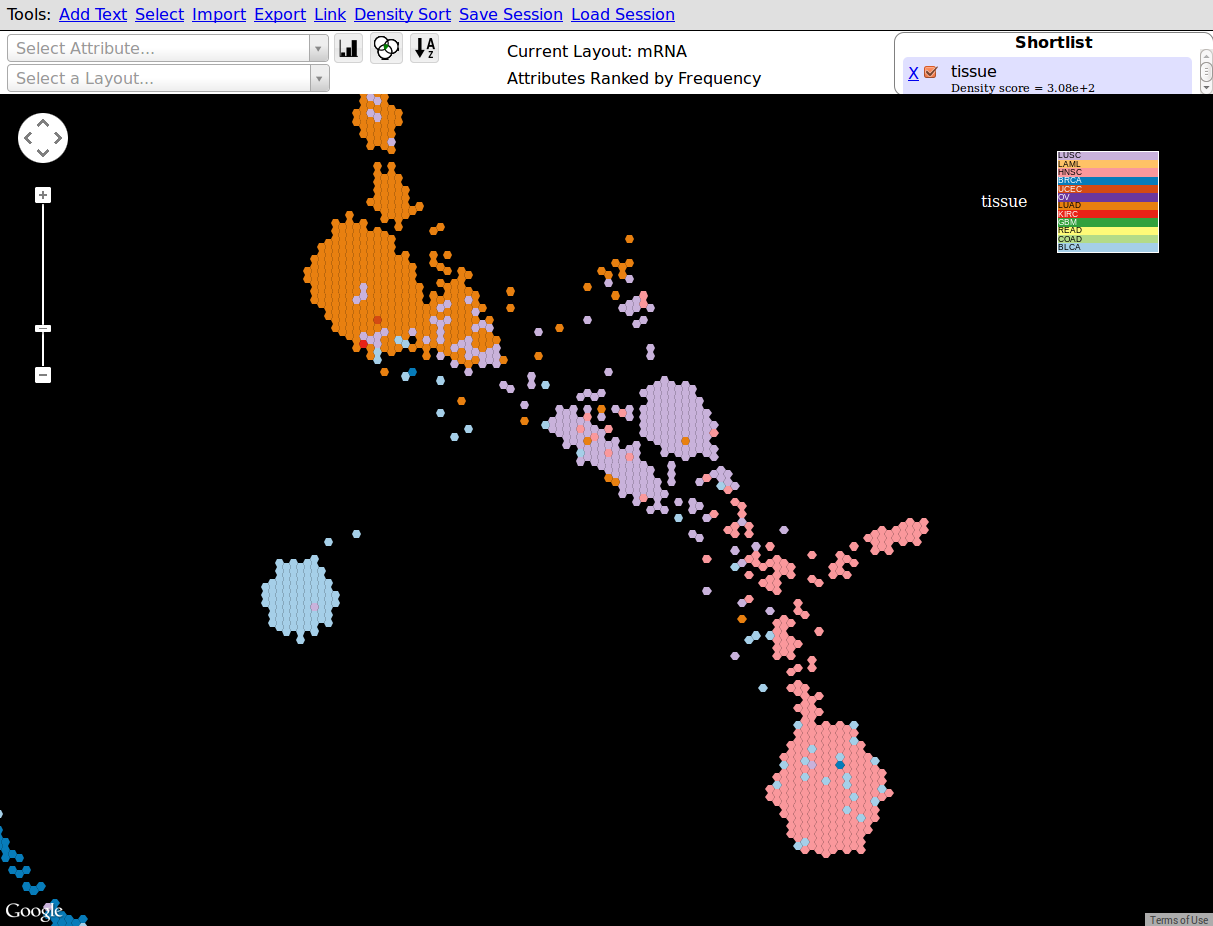
\includegraphics[width=1.0\textwidth]{figures/tumormap.png}
    \caption{A screenshot of the UCSC Tumor Map. Individual tumor samples are represented by cells in a hexagonal grid, laid out using a spring layout algorithm based on molecular similarity. The map is browseable using a Google Maps interface. Hexes can be colored using various data overlays, and statistical queries can be run interactively.}
    \label{fig:tumormap}
\end{figure}

The visualization itself consists of a hexagonal grid on which tumor samples are arranged, with at most one sample in each cell. Samples are arranged according to sample-sample similarity values from a similarity matrix, which are then used as spring strengths in the DrL graph spring layout algorithm \cite{martin2008drl}. If the cell a sample would occupy is already filled, it is placed in a minimally distant free cell. This algorithm is found to produce ``islands'' of similar samples, with some interaction between and substructure within them.

The hexagonal grid is conceptually a map: tumor samples are placed near other samples that they are similar to, and far from samples that they are very different from. This creates a two-dimensional space in which scientists can form and test hypotheses about what features drive these similarities and differences. To aid in this process, the Tumor Map provides a facility for displaying attribute overlays, allowing continuous, binary, or categorical per-sample data to be visualized in this space. By default, the visualization displays a tissue overlay, coloring each sample according to the tissue from which the tumor was originally derived. Other attribute overlays depicting per-tumor characteristics like mutations in important cancer genes, or the relative levels of activation of various transcriptional programs, can be brought up using the dropdown in the upper left. Up to two can be displayed at a time, using a dynamically-generated color scheme.

The visualization provides facilities for running statistical tests on the attribute overlays. When the visualization is first opened, attributes are sorted by a layout-aware density metric, with attributes that have particularly high or low values significantly clustered together in the space defined by the map being sorted to the top of the list. Other statistical tests available include layout-aware and layout-independent association tests, to find other attributes statistically significantly related to a ``pivot'' attribute, and a dichotomy-based sort to find attributes that are statistically significantly different between two user-selected groups of samples. Using these tools, scientists can quickly ask and answer questions like ``what's special about this little clump of tumors budding off from this island?'' or ``what other kinds of tumors look like TP53-mutated tumors in this space?''.

The current official version is built against the TCGA PanCancer data set, with a variety of locally-produced and imported overlays, but the code to generate the visualization is implemented as a Galaxy tool, and can be used to generate a visualization from any appropriately formatted similarity matrix and set of overlays \cite{weinstein2013cancer,giardine2005galaxy}. The full details about the data that went into the current sample visualization, as well as more information on the algorithms used, can be found in \cite{novak2014ucsc}.

The UCSC Tumor Map is worth mentioning here primarily because, anecdotally, scientists appear to enjoy using it. Its primary focus is bringing the concept of space to pan-cancer tumor analysis, and, whether or not it ever gets used to discover an important novel result, it is clear that scientists want to be able to use spatial thinking to understand datasets. This lesson on the importance of spatial metaphors will be applied in the development of the graph-based genome representations that are proposed here.

% I made a pan-cancer visualization of the entire cross-tissue TCGA data set
    
    % Lay out all the tumors by a similarity metric, and squish them into a hexagonal grid in 2D
    
    % Let people fly around it with Google Maps
    
    % Then draw map overlays depicting various tumor or patient attributes.

    % Less a scaling up of the analysis than a scaling down of the data set into a space where people are comfortable working.
    
% See the paper. 

\section{Project \#2: NOTCH2NL Copy Number Variation Analysis}

A graph-based analysis of NOTCH2NL paralog copy number is a second and somewhat more relevant piece of prior work. As discussed above, while the older GRCh37 assembly had only a single NOTCH2NL gene annotated, new information from sequencing haploid cells (from a hyatidiform mole) revealed the existence of four paralogs, here dubbed NOTCH2NL-A, NOTCH2NL-B, NOTCH2NL-C, and NOTCH2NL-D \cite{jacobs2014recently}. Moreover, NOTCH2NL-A, -B, and -C were found to be located quite close to ``the 1q21.1 distal deletion/duplication locus'', copy number variations of which have been associated with congenital microcephaly and macrocephaly \cite{jacobs2014recently}. The goal of the project was to determine if deletions or duplications of any of the nearby NOTCH2NL genes could potentially explain these microcephalic and macrocephalic phenotypes.

Several approaches were taken to attempt to answer this question, including experimental wet-lab characterization of the NOTCH2NL proteins' effects in mice and reanalysis of high-throughput-sequencing data to try to look for copy number variations in these genes in the general population \cite{jacobs2014recently}. The approach that represents prior work for the current proposal, however, relied on a collection of DNA microarrays from people with microcephaly, people with macrocephaly, and people with neither condition.

The microarrays provided comparative genomic hybridization (CGH) data: for each probe, the array gave what was supposed to be the ratio of the amount of matching DNA in the sample to the amount of matching DNA in a standard ``normal'' genome. As microarrays were involved, so was a tedious amount of normalization, which is described in full in the supplement of \cite{jacobs2014recently}. Briefly, the analysis pipeline worked by first re-mapping the sequences of the microarray probes to the hyatidiform mole assembly with pblat, and taking all hits \cite{meng2012parallelized}. Probes that had no mapping locations near the region of interest were ignored. The relative affinity of each probe for hybridizing with each of its mapping locations was calculated using DECIPHER \cite{wright2012decipher}.

This information on probe mapping locations was used to create a graphical integer linear programming (ILP) model of the sample and standard normal genomes. Each probe mapping location became two graph nodes, one representing its copy number in the sample, and one representing its copy number in the standard normal genome (which may have itself had copy number differences relative to the hyatidiform mole assembly). Each mapping location in each genome had a linear programming variable representing its copy number, and constraints were added penalizing copy number differences between adjacent probe mapping locations. For each probe, all of its mapping locations in each genome were linked together in an affinity-weighted sum representing the total hybridization of that probe in that genome; the hybridization levels of each probe in each genome were constrained together to penalize deviation from the observed microarray hybridization ratios for the sample being analyzed (after normalizing against a series of control samples for the array, if available). Additionally, all copy number estimates were slightly penalized for deviations from the ordinarily expected value of 2 copies, which is generally what copy number is in a diploid genome. Each sample's linear programming problem was solved with the CBC linear programming solver, finding optimal copy numbers for each probe mapping location in each genome under the constraints imposed by the graph. The process was repeated with different linear programming constraint weights in order to distinguish high- and low-confidence copy number changes \cite{forrest2013cbc}.

\begin{figure}[ht]
    \centering
    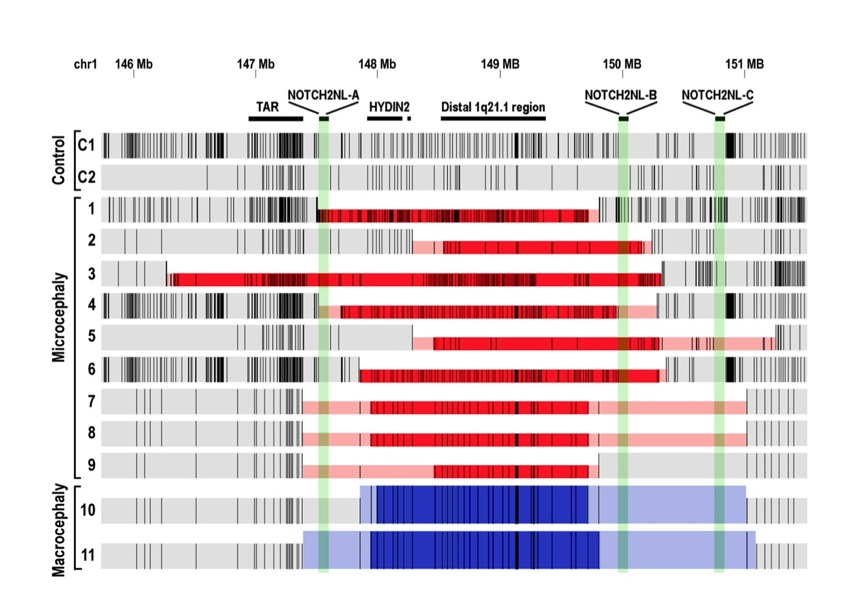
\includegraphics[width=1.0\textwidth]{figures/notch2nl.png}
    \caption{Linear-programming-based copy number inference pipeline results for patients with microcephaly (red), patients with macrocephaly (blue), and control patients. Regions which are potentially (light) or with high confidence (dark) altered in copy number are highlighted. Black lines show linear-programming-processed copy numbers at microarray probe binding locations. NOTCH2NL-B copy number is reduced with high confidence in 4 of 8 patients with microcephaly. NOTCH2NL-A copy number is reduced with high confidence in 2 of 8 patients with microcephaly. The dataset is consistent with at least one copy of NOTCH2NL-A or NOTCH2NL-B being deleted in each microcephaly patient, and at least one being duplicated in each macrocephaly patient. No copy number alterations were detected in any of the NOTCH2NL genes for any of the controls. Adapted from \cite{jacobs2014recently} Figure 5B.}
    \label{fig:notch2nl}
\end{figure}

The results of this process are visible in Figure \ref{fig:notch2nl}. Copy number changes were found in the region of interest in all of the microcephaly and macrocephaly patients examined, and in none of the controls. Moreover, all of the copy number changes in microcephaly patients are consistent with a deletion of NOTCH2NL-A or NOTCH2NL-B (or both), and likewise the copy number changes in the two macrocephaly patients are consistent with similar duplications. Unfortunately, the NOTCH2NL genes do not always fall in the regions where copy number was determined to have been altered with high confidence; this only happens in 4 of the 8 microcephaly patients, and neither of the macrocephaly patients. However, this is in part due to the sparsity of probe mapping locations in the vicinities of the NOTCH2NL genes, where the hyatidiform mole assembly provides new sequence relative to previous assemblies.

This prior work is important for the project being proposed now because it illustrates the usefulness of graphical models of genomes and of genomic variation. The use of a graphical model here allowed information to be extracted from microarray probes which did not unambiguously map to only a single location in the genome, which in turn allowed microarray data from arrays designed on older references to be effectively used with a new custom reference. Furthermore, several seemingly distinct structural variants were uncovered in the region examined here. Although they may be private to the individuals in this study, it is clear that, if one wanted to store them in some sort of database of variation, one would need a way to effectively represent distinct, partially overlapping structural variants---a task for which graph representations are well-suited.



% I made a first pass at analyzing the NOTCH2NL region
    
    % I specifically worked on a linear programming based approach to make copy number calls on our corrected assembly using CGH microarray probes originally designed for an assembly that conflated the NOTCH2NL genes
    
    % Trying to handle multimapping, because if I threw out multimapping I would have thrown out XX% of the data.
        
        % This again isn't really scaling, but it's something we need to do to support scaling.
    
% We found that CNV in the NOTCH2NL region can explain disease.

    % See the paper.

\section{Project \#3: Mapping to a Reference Genome Structure}

In order to implement any sort of new data structure, it is necessary to work out what operations the structure is to support and how those algorithms are supposed to work. To that end, as a preliminary to the work proposed here, a rigorous mathematical model of ``reference structures'' and their associated operations \cite{paten2014mapping}. 

% TODO: This section is lifted from the paper and needs to fit in with the rest (i.e. match in person and stuff).

We model both reference and individual genome assemblies as \vocab{sequence graphs}, which allow for a more general class of assembly representation, and which incorporate phased contig/scaffold representations as a special case. 

A \vocab{base instance} is a pair $(b,P)$ consisting of a labeling base $b$ in $\{\mathrm{A},\mathrm{C},\mathrm{T},\mathrm{G}\}$ and a \vocab{position} $P$. All positions are globally unique, so given a position $P$, one may determine the base at that position, i.e. the unique $b$ such that $(b,P)$ is a base instance. The nucleotides in all genomes are described as base instances. 

In order to define a sequence graph, we need to specify how base instances are connected to form sequences. To do this generally, as DNA is double stranded, we must distinguish the forward and reverse complement orientations of base instances. Each base instance $(b,P)$ has a \vocab{left side}, denoted $P_l$, and a \vocab{right side}, denoted $P_r$. An \vocab{adjacency} is an unordered pair of two sides; an adjacency ${P_s, Q_t}$ asserts that the $s$ side of the base at position $P$ is connected to the $t$ side of the base at position $Q$. 

A \vocab{sequence graph} $G = (V_G,E_G)$ is a bidirected graph \cite{medvedev2009maximum} in which each node in the set $V_G$ of nodes is a base instance and each edge in the set $E_G$ of edges is an adjacency connecting the sides of two base instances. The forward label of a node $(b,P)$ is the base $b$, and the reverse label is the reverse complement base $b*$, where $\mathrm{A}* = \mathrm{T}$, $\mathrm{T}* = \mathrm{A}$, $\mathrm{G}* = \mathrm{C}$, and $\mathrm{C}* = \mathrm{G}$. Using its sides for orientation, for a base instance $(b, P)$ we write $b(P_l) = b$ and $b(P_r) = b*$ to denote the base label oriented by the given side.

A \vocab{linear thread} is a special kind of path in a sequence graph composed of a sequence of oriented nodes and edges terminated by oriented nodes, such that each node other than the first and last node on the path is entered on one side and exited on the other. Nodes can be visited more than once in a thread. The traversal of a thread specifies a sequence of nucleotides, decoded by enumerating the labels of base instances in the order and orientation specified by the thread, such that if a base instance $(b, P)$ is oriented from $P_l$ to $P_r$ then $b(P_l) = b$ is incorporated into the traversal, and if oriented from $P_r$  to $P_l$  then $b(P_r) = b*$ is incorporated into the traversal. A \vocab{circular thread} is a circular path of oriented nodes and edges in which each node is entered on one side and exited on the other. Its traversal is a circular sequence of nucleotides, like a mitochondrial or bacterial sequence.  

A \vocab{contig graph}, or \vocab{contig}, is a sequence graph that consists of a single linear or circular thread with no node repetitions. A phased sequence graph is a sequence graph consisting of a set of disjoint contig subgraphs.

Any sequence graph that is not a phased sequence graph is called \vocab{unphased}. Unphased sequence graphs can be used to represent genomes in which there is some uncertainty in phasing or assembly. They can also be used to represent populations of genomes in which numerous variations are described, e.g. an extension of a reference genome assembly to include more than one variant of some regions

Let us assume that we are given an input sequence graph $G$ and a target sequence graph $H$. The task is to map the input base instances in $V_G$ to corresponding target base instances in $V_H$. Often the input graph will represent the genome of a particular individual and the target graph will be used as a reference genome. To avoid wrongly categorizing genetic variations in the input graph, we leave a base instance in $V_G$ unmapped if it can plausibly map to more than one base instance in $V_H$. The mapping may therefore be partial; i.e. it is not assumed that all elements of VG will be mapped. Since the identifier $P$ of the base instance $(b,P)$ determines the base $b$, it suffices to map positions uniquely to positions, i.e. identifiers to identifiers. However, to account for the double-sided nature of DNA strands, we must allow a position $P$ in $G$ to map to a position in $H$ in either the forward or reverse orientation. Formally, a mapping from a sequence graph $G$ to a sequence graph $H$ is a partial function $M$ from the set of positions in $G$ to the set of positions in $H$ such that for every position $P$ in $G$, either $M(P)$ is undefined and we say that position $P$ is \vocab{unmapped} in $H$, or there is a position $Q$ in $H$ such that $M(P) = Q$ and either $b(P_l) = b(Q_l)$ (and we say that $P$ is \vocab{forward mapped} to $Q$ in $H$), or $b(P_l) = b(Q_r)$ (and we say that $P$ is \vocab{reverse mapped} to $Q$ in $H$). In either of the latter two cases we say that position $P$ \vocab{maps} to the position $Q$ in $H$ (or more generally that the position $P$ is mapped in $H$).  

Let $H$ be a phased sequence graph to be treated as a target (e.g. reference) genome. For each side $Q_s$ in $H$ the \vocab{unique context} of $Q_s$, denoted $U(Q_s)$, is the shortest suffix $u$ of the traversal of a thread in $H$ ending at $Q$ entered from its $s$ side, such that $u$ occurs exactly once as a traversal of a thread in $H$ (ending at any side of any node). The suffix $u$ includes the base of $Q$, and does not always include other bases. If no such unique suffix $u$ exists for $Q_s$, we say that the side $Q_s$ is \vocab{unmappable} (Fig. 4).

For a side $P_s$ in a phased sequence graph $G$, $P_s$ is matched to a side $Q_t$ in a phased target sequence graph $H$ if a suffix of the traversal of the thread ending at and including $P$ entered from its s side is the same as $U(Q_t)$. The essential property of the unique contexts of $H$ is that, as a family, they don’t share suffixes, which means any side in any $G$ can be matched to at most one side in $H$. 

Given the above matching of sides, the left-right exact match mapping $M_e$ of positions is defined as follows; a position $P$ in $G$ is:
\begin{itemize}
\item unmapped in $H$ (and $M_e(P)$ is undefined) if neither $P_l$ or $P_r$ are matched anywhere, 
\item \vocab{left-mapped} at $M_e(P) = Q$ if $P_l$  is matched to a side of $Q$, but $P_r$  is not matched anywhere, 
\item \vocab{right-mapped} at $M_e(P) = Q$ if $P_r$ is matched to a side of $Q$, but $P_l$ is not matched anywhere,
\item \vocab{fully-mapped} at $M_e(P) = Q$ if $P_l$  is matched to one side of $Q$ and $P_r$ is matched to the other side of $Q$,
\item else $P$ is \vocab{inconsistently-mapped} in $H$ (and $M_e(P)$ is undefined).
\end{itemize}

Combining cases, we say that position $P$ is mapped in $H$ if it is left-mapped, right-mapped or fully-mapped, and not mapped in $H$ if is it either unmapped or inconsistently-mapped. This defines the left-right exact match mapping $M_e$ from $G$ to $H$. 

A toy example of a reference structure is given in Figure \ref{fig:lrexactmatch}.

\begin{figure}[ht]
    \centering
    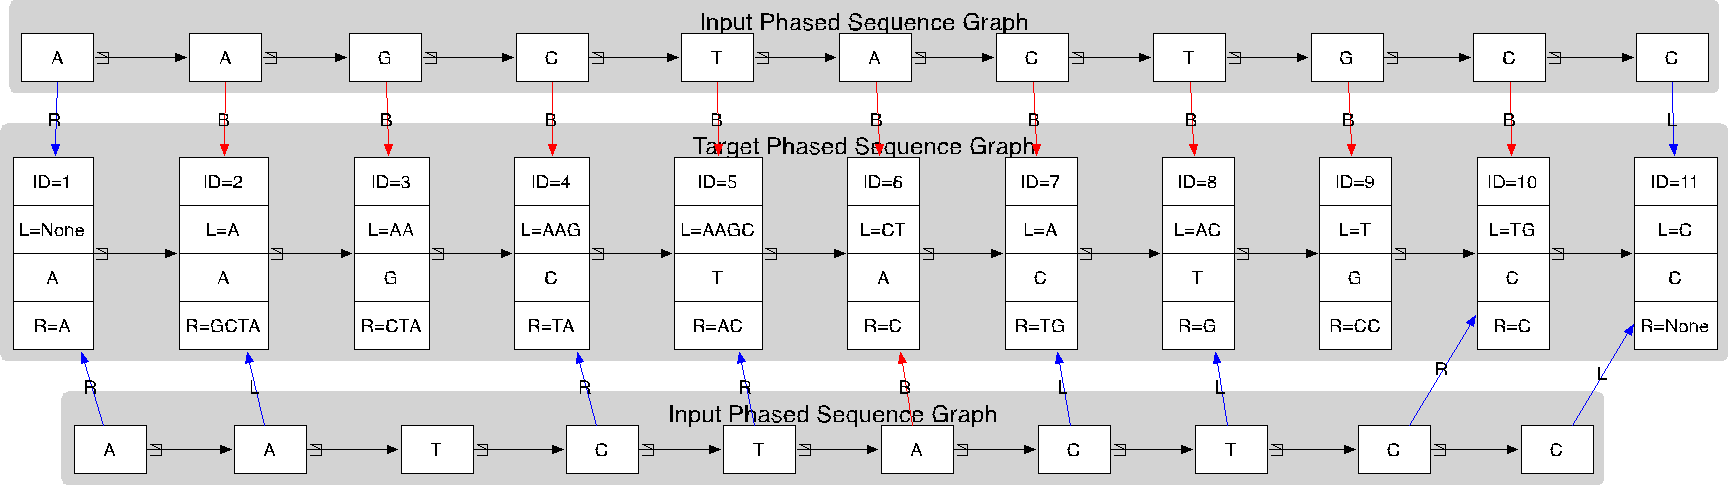
\includegraphics[width=1.0\textwidth]{figures/lrexactmatch.png}
    \caption{An example of two query sequences (top and bottom) being mapped to a reference structure (middle) by the Left-Right Exact Match mapping scheme.}
    \label{fig:lrexactmatch}
\end{figure}

A full description of reference structure theory is available in \cite{paten2014mapping}.


% We developed a rigorous theory for making reference graphs, putting them in hierarchies, and mapping to them based on context.

% I'm going to need this in my system as an alternative to linear coordinates, since linear coordinates have all the problems mentioned above.

% The hierarchy stuff is also how I plan to formalize multimapping into something useful.

% See the paper.

\chapter{Proposed Work}

\section{Specific Aim \#1: Develop Reference Hierarchy Theory}

% I need a rigorous theory of reference structures, reference hierarchies, mapping, and multimapping

% Also a mathematics of variants as paths, and a reference as a collection of equal variants.

% This is mostly completed, but we're working on new and exciting things like mapping on credit.

\section{Specific Aim \#2: Engineer Scalable Software Tools}

% I need to turn Specific Aim #1 from math into software.

% To be minimally useful it needs to be able to do at least what we do now: map to hg38 plus alt haplotypes
    
    % But in a graph-based way
    
% So far I've implemented this for the hg38 MHC region.
    
% What I actually want to do is to be able to map to hg38 and alts, plus a bunch of other variants.

    % I'd like to show that this reduces reference bias in mapping
    
% I don't plan to scale to more than tens of genomes' worth of sequence in the reference within the scope of this project.

    % I can fit a bunch of examples of variants in without full genomes to hold them.
    
% I'm going to stick an API on it so the software is accessible from multiple languages

    % Ideally with RPC so you don't need to mirror this whole graph structure in order to slice it and look up variants.

\section{Specific Aim \#3: Discover Biologically Relevant Variation}

% Once I've built the system, I'll browse around the graph and see if I can find anything interesting.

% Since this system will be well-designed for analyzing structural variants, I will see if I can compile some broad statistics about the number and type of structural variants in my reference versus in other compendiums of structural variation.

% If I can't find anything else, I could take another look at the NOTCH2NL region, and repeat my analysis of the CGH microarray data in graph terms.

\appendix
\chapter{Some Ancillary Stuff}

Ancillary material should be put in appendices, which appear BEFORE the
bibliography. 

% %%%%%%%%%%%%%%%%%%%%%%%%%%%%%%%%%%%%%%%%%%%%%%%%%%%%%%%%%
% bibliography

% 2010june01 sol katzman:
% if \nocite is specified, all entries in the bib file are included,
% probably not what you want, so comment out the \nocite and only get the cited references.
\nocite{*}

% 2010june01 sol katzman:
% this makes the bibliography single spaced, with double spacing between entries
\def\baselinestretch{1.0}\large\normalsize

\bibliographystyle{plain}
\bibliography{proposal}

\end{document}
